
%% bare_jrnl_compsoc.tex
%% V1.4a
%% 2014/09/17
%% by Michael Shell
%% See:
%% http://www.michaelshell.org/
%% for current contact information.
%%
%% This is a skeleton file demonstrating the use of IEEEtran.cls
%% (requires IEEEtran.cls version 1.8a or later) with an IEEE
%% Computer Society journal paper.
%%
%% Support sites:
%% http://www.michaelshell.org/tex/ieeetran/
%% http://www.ctan.org/tex-archive/macros/latex/contrib/IEEEtran/
%% and
%% http://www.ieee.org/

%%*************************************************************************
%% Legal Notice:
%% This code is offered as-is without any warranty either expressed or
%% implied; without even the implied warranty of MERCHANTABILITY or
%% FITNESS FOR A PARTICULAR PURPOSE! 
%% User assumes all risk.
%% In no event shall IEEE or any contributor to this code be liable for
%% any damages or losses, including, but not limited to, incidental,
%% consequential, or any other damages, resulting from the use or misuse
%% of any information contained here.
%%
%% All comments are the opinions of their respective authors and are not
%% necessarily endorsed by the IEEE.
%%
%% This work is distributed under the LaTeX Project Public License (LPPL)
%% ( http://www.latex-project.org/ ) version 1.3, and may be freely used,
%% distributed and modified. A copy of the LPPL, version 1.3, is included
%% in the base LaTeX documentation of all distributions of LaTeX released
%% 2003/12/01 or later.
%% Retain all contribution notices and credits.
%% ** Modified files should be clearly indicated as such, including  **
%% ** renaming them and changing author support contact information. **
%%
%% File list of work: IEEEtran.cls, IEEEtran_HOWTO.pdf, bare_adv.tex,
%%                    bare_conf.tex, bare_jrnl.tex, bare_conf_compsoc.tex,
%%                    bare_jrnl_compsoc.tex, bare_jrnl_transmag.tex
%%*************************************************************************


% *** Authors should verify (and, if needed, correct) their LaTeX system  ***
% *** with the testflow diagnostic prior to trusting their LaTeX platform ***
% *** with production work. IEEE's font choices and paper sizes can       ***
% *** trigger bugs that do not appear when using other class files.       ***                          ***
% The testflow support page is at:
% http://www.michaelshell.org/tex/testflow/


\documentclass[10pt,journal,compsoc]{IEEEtran}
%
% If IEEEtran.cls has not been installed into the LaTeX system files,
% manually specify the path to it like:
% \documentclass[10pt,journal,compsoc]{../sty/IEEEtran}





% Some very useful LaTeX packages include:
% (uncomment the ones you want to load)


% *** MISC UTILITY PACKAGES ***
%
%\usepackage{ifpdf}
% Heiko Oberdiek's ifpdf.sty is very useful if you need conditional
% compilation based on whether the output is pdf or dvi.
% usage:
% \ifpdf
%   % pdf code
% \else
%   % dvi code
% \fi
% The latest version of ifpdf.sty can be obtained from:
% http://www.ctan.org/tex-archive/macros/latex/contrib/oberdiek/
% Also, note that IEEEtran.cls V1.7 and later provides a builtin
% \ifCLASSINFOpdf conditional that works the same way.
% When switching from latex to pdflatex and vice-versa, the compiler may
% have to be run twice to clear warning/error messages.






% *** CITATION PACKAGES ***
%
\ifCLASSOPTIONcompsoc
  % IEEE Computer Society needs nocompress option
  % requires cite.sty v4.0 or later (November 2003)
  \usepackage[nocompress]{cite}
\else
  % normal IEEE
  \usepackage{cite}
\fi
% cite.sty was written by Donald Arseneau
% V1.6 and later of IEEEtran pre-defines the format of the cite.sty package
% \cite{} output to follow that of IEEE. Loading the cite package will
% result in citation numbers being automatically sorted and properly
% "compressed/ranged". e.g., [1], [9], [2], [7], [5], [6] without using
% cite.sty will become [1], [2], [5]--[7], [9] using cite.sty. cite.sty's
% \cite will automatically add leading space, if needed. Use cite.sty's
% noadjust option (cite.sty V3.8 and later) if you want to turn this off
% such as if a citation ever needs to be enclosed in parenthesis.
% cite.sty is already installed on most LaTeX systems. Be sure and use
% version 5.0 (2009-03-20) and later if using hyperref.sty.
% The latest version can be obtained at:
% http://www.ctan.org/tex-archive/macros/latex/contrib/cite/
% The documentation is contained in the cite.sty file itself.
%
% Note that some packages require special options to format as the Computer
% Society requires. In particular, Computer Society  papers do not use
% compressed citation ranges as is done in typical IEEE papers
% (e.g., [1]-[4]). Instead, they list every citation separately in order
% (e.g., [1], [2], [3], [4]). To get the latter we need to load the cite
% package with the nocompress option which is supported by cite.sty v4.0
% and later. Note also the use of a CLASSOPTION conditional provided by
% IEEEtran.cls V1.7 and later.





% *** GRAPHICS RELATED PACKAGES ***
%
\ifCLASSINFOpdf
  % \usepackage[pdftex]{graphicx}
  % declare the path(s) where your graphic files are
  % \graphicspath{{../pdf/}{../jpeg/}}
  % and their extensions so you won't have to specify these with
  % every instance of \includegraphics
  % \DeclareGraphicsExtensions{.pdf,.jpeg,.png}
\else
  % or other class option (dvipsone, dvipdf, if not using dvips). graphicx
  % will default to the driver specified in the system graphics.cfg if no
  % driver is specified.
  % \usepackage[dvips]{graphicx}
  % declare the path(s) where your graphic files are
  % \graphicspath{{../eps/}}
  % and their extensions so you won't have to specify these with
  % every instance of \includegraphics
  % \DeclareGraphicsExtensions{.eps}
\fi
% graphicx was written by David Carlisle and Sebastian Rahtz. It is
% required if you want graphics, photos, etc. graphicx.sty is already
% installed on most LaTeX systems. The latest version and documentation
% can be obtained at: 
% http://www.ctan.org/tex-archive/macros/latex/required/graphics/
% Another good source of documentation is "Using Imported Graphics in
% LaTeX2e" by Keith Reckdahl which can be found at:
% http://www.ctan.org/tex-archive/info/epslatex/
%
% latex, and pdflatex in dvi mode, support graphics in encapsulated
% postscript (.eps) format. pdflatex in pdf mode supports graphics
% in .pdf, .jpeg, .png and .mps (metapost) formats. Users should ensure
% that all non-photo figures use a vector format (.eps, .pdf, .mps) and
% not a bitmapped formats (.jpeg, .png). IEEE frowns on bitmapped formats
% which can result in "jaggedy"/blurry rendering of lines and letters as
% well as large increases in file sizes.
%
% You can find documentation about the pdfTeX application at:
% http://www.tug.org/applications/pdftex






% *** MATH PACKAGES ***
%
%\usepackage[cmex10]{amsmath}
% A popular package from the American Mathematical Society that provides
% many useful and powerful commands for dealing with mathematics. If using
% it, be sure to load this package with the cmex10 option to ensure that
% only type 1 fonts will utilized at all point sizes. Without this option,
% it is possible that some math symbols, particularly those within
% footnotes, will be rendered in bitmap form which will result in a
% document that can not be IEEE Xplore compliant!
%
% Also, note that the amsmath package sets \interdisplaylinepenalty to 10000
% thus preventing page breaks from occurring within multiline equations. Use:
%\interdisplaylinepenalty=2500
% after loading amsmath to restore such page breaks as IEEEtran.cls normally
% does. amsmath.sty is already installed on most LaTeX systems. The latest
% version and documentation can be obtained at:
% http://www.ctan.org/tex-archive/macros/latex/required/amslatex/math/





% *** SPECIALIZED LIST PACKAGES ***
%
%\usepackage{algorithmic}
% algorithmic.sty was written by Peter Williams and Rogerio Brito.
% This package provides an algorithmic environment fo describing algorithms.
% You can use the algorithmic environment in-text or within a figure
% environment to provide for a floating algorithm. Do NOT use the algorithm
% floating environment provided by algorithm.sty (by the same authors) or
% algorithm2e.sty (by Christophe Fiorio) as IEEE does not use dedicated
% algorithm float types and packages that provide these will not provide
% correct IEEE style captions. The latest version and documentation of
% algorithmic.sty can be obtained at:
% http://www.ctan.org/tex-archive/macros/latex/contrib/algorithms/
% There is also a support site at:
% http://algorithms.berlios.de/index.html
% Also of interest may be the (relatively newer and more customizable)
% algorithmicx.sty package by Szasz Janos:
% http://www.ctan.org/tex-archive/macros/latex/contrib/algorithmicx/




% *** ALIGNMENT PACKAGES ***
%
%\usepackage{array}
% Frank Mittelbach's and David Carlisle's array.sty patches and improves
% the standard LaTeX2e array and tabular environments to provide better
% appearance and additional user controls. As the default LaTeX2e table
% generation code is lacking to the point of almost being broken with
% respect to the quality of the end results, all users are strongly
% advised to use an enhanced (at the very least that provided by array.sty)
% set of table tools. array.sty is already installed on most systems. The
% latest version and documentation can be obtained at:
% http://www.ctan.org/tex-archive/macros/latex/required/tools/


% IEEEtran contains the IEEEeqnarray family of commands that can be used to
% generate multiline equations as well as matrices, tables, etc., of high
% quality.




% *** SUBFIGURE PACKAGES ***
%\ifCLASSOPTIONcompsoc
%  \usepackage[caption=false,font=footnotesize,labelfont=sf,textfont=sf]{subfig}
%\else
%  \usepackage[caption=false,font=footnotesize]{subfig}
%\fi
% subfig.sty, written by Steven Douglas Cochran, is the modern replacement
% for subfigure.sty, the latter of which is no longer maintained and is
% incompatible with some LaTeX packages including fixltx2e. However,
% subfig.sty requires and automatically loads Axel Sommerfeldt's caption.sty
% which will override IEEEtran.cls' handling of captions and this will result
% in non-IEEE style figure/table captions. To prevent this problem, be sure
% and invoke subfig.sty's "caption=false" package option (available since
% subfig.sty version 1.3, 2005/06/28) as this is will preserve IEEEtran.cls
% handling of captions.
% Note that the Computer Society format requires a sans serif font rather
% than the serif font used in traditional IEEE formatting and thus the need
% to invoke different subfig.sty package options depending on whether
% compsoc mode has been enabled.
%
% The latest version and documentation of subfig.sty can be obtained at:
% http://www.ctan.org/tex-archive/macros/latex/contrib/subfig/




% *** FLOAT PACKAGES ***
%
%\usepackage{fixltx2e}
% fixltx2e, the successor to the earlier fix2col.sty, was written by
% Frank Mittelbach and David Carlisle. This package corrects a few problems
% in the LaTeX2e kernel, the most notable of which is that in current
% LaTeX2e releases, the ordering of single and double column floats is not
% guaranteed to be preserved. Thus, an unpatched LaTeX2e can allow a
% single column figure to be placed prior to an earlier double column
% figure. The latest version and documentation can be found at:
% http://www.ctan.org/tex-archive/macros/latex/base/


%\usepackage{stfloats}
% stfloats.sty was written by Sigitas Tolusis. This package gives LaTeX2e
% the ability to do double column floats at the bottom of the page as well
% as the top. (e.g., "\begin{figure*}[!b]" is not normally possible in
% LaTeX2e). It also provides a command:
%\fnbelowfloat
% to enable the placement of footnotes below bottom floats (the standard
% LaTeX2e kernel puts them above bottom floats). This is an invasive package
% which rewrites many portions of the LaTeX2e float routines. It may not work
% with other packages that modify the LaTeX2e float routines. The latest
% version and documentation can be obtained at:
% http://www.ctan.org/tex-archive/macros/latex/contrib/sttools/
% Do not use the stfloats baselinefloat ability as IEEE does not allow
% \baselineskip to stretch. Authors submitting work to the IEEE should note
% that IEEE rarely uses double column equations and that authors should try
% to avoid such use. Do not be tempted to use the cuted.sty or midfloat.sty
% packages (also by Sigitas Tolusis) as IEEE does not format its papers in
% such ways.
% Do not attempt to use stfloats with fixltx2e as they are incompatible.
% Instead, use Morten Hogholm'a dblfloatfix which combines the features
% of both fixltx2e and stfloats:
%
% \usepackage{dblfloatfix}
% The latest version can be found at:
% http://www.ctan.org/tex-archive/macros/latex/contrib/dblfloatfix/




%\ifCLASSOPTIONcaptionsoff
%  \usepackage[nomarkers]{endfloat}
% \let\MYoriglatexcaption\caption
% \renewcommand{\caption}[2][\relax]{\MYoriglatexcaption[#2]{#2}}
%\fi
% endfloat.sty was written by James Darrell McCauley, Jeff Goldberg and 
% Axel Sommerfeldt. This package may be useful when used in conjunction with 
% IEEEtran.cls'  captionsoff option. Some IEEE journals/societies require that
% submissions have lists of figures/tables at the end of the paper and that
% figures/tables without any captions are placed on a page by themselves at
% the end of the document. If needed, the draftcls IEEEtran class option or
% \CLASSINPUTbaselinestretch interface can be used to increase the line
% spacing as well. Be sure and use the nomarkers option of endfloat to
% prevent endfloat from "marking" where the figures would have been placed
% in the text. The two hack lines of code above are a slight modification of
% that suggested by in the endfloat docs (section 8.4.1) to ensure that
% the full captions always appear in the list of figures/tables - even if
% the user used the short optional argument of \caption[]{}.
% IEEE papers do not typically make use of \caption[]'s optional argument,
% so this should not be an issue. A similar trick can be used to disable
% captions of packages such as subfig.sty that lack options to turn off
% the subcaptions:
% For subfig.sty:
% \let\MYorigsubfloat\subfloat
% \renewcommand{\subfloat}[2][\relax]{\MYorigsubfloat[]{#2}}
% However, the above trick will not work if both optional arguments of
% the \subfloat command are used. Furthermore, there needs to be a
% description of each subfigure *somewhere* and endfloat does not add
% subfigure captions to its list of figures. Thus, the best approach is to
% avoid the use of subfigure captions (many IEEE journals avoid them anyway)
% and instead reference/explain all the subfigures within the main caption.
% The latest version of endfloat.sty and its documentation can obtained at:
% http://www.ctan.org/tex-archive/macros/latex/contrib/endfloat/
%
% The IEEEtran \ifCLASSOPTIONcaptionsoff conditional can also be used
% later in the document, say, to conditionally put the References on a 
% page by themselves.




% *** PDF, URL AND HYPERLINK PACKAGES ***
%
\usepackage{url}
% url.sty was written by Donald Arseneau. It provides better support for
% handling and breaking URLs. url.sty is already installed on most LaTeX
% systems. The latest version and documentation can be obtained at:
% http://www.ctan.org/tex-archive/macros/latex/contrib/url/
% Basically, \url{my_url_here}.

\usepackage[utf8]{inputenc}
\usepackage[T1]{fontenc}
\usepackage[spanish]{babel}
\usepackage{graphicx}
\usepackage{booktabs}
\graphicspath{ {images/} }



% *** Do not adjust lengths that control margins, column widths, etc. ***
% *** Do not use packages that alter fonts (such as pslatex).         ***
% There should be no need to do such things with IEEEtran.cls V1.6 and later.
% (Unless specifically asked to do so by the journal or conference you plan
% to submit to, of course. )


% correct bad hyphenation here
\hyphenation{op-tical net-works semi-conduc-tor}


\begin{document}
%
% paper title
% Titles are generally capitalized except for words such as a, an, and, as,
% at, but, by, for, in, nor, of, on, or, the, to and up, which are usually
% not capitalized unless they are the first or last word of the title.
% Linebreaks \\ can be used within to get better formatting as desired.
% Do not put math or special symbols in the title.
\title{Wi-Fi, WiMAX y LiFi}
%
%
% author names and IEEE memberships
% note positions of commas and nonbreaking spaces ( ~ ) LaTeX will not break
% a structure at a ~ so this keeps an author's name from being broken across
% two lines.
% use \thanks{} to gain access to the first footnote area
% a separate \thanks must be used for each paragraph as LaTeX2e's \thanks
% was not built to handle multiple paragraphs
%
%
%\IEEEcompsocitemizethanks is a special \thanks that produces the bulleted
% lists the Computer Society journals use for "first footnote" author
% affiliations. Use \IEEEcompsocthanksitem which works much like \item
% for each affiliation group. When not in compsoc mode,
% \IEEEcompsocitemizethanks becomes like \thanks and
% \IEEEcompsocthanksitem becomes a line break with idention. This
% facilitates dual compilation, although admittedly the differences in the
% desired content of \author between the different types of papers makes a
% one-size-fits-all approach a daunting prospect. For instance, compsoc 
% journal papers have the author affiliations above the "Manuscript
% received ..."  text while in non-compsoc journals this is reversed. Sigh.



% note the % following the last \IEEEmembership and also \thanks - 
% these prevent an unwanted space from occurring between the last author name
% and the end of the author line. i.e., if you had this:
% 
% \author{....lastname \thanks{...} \thanks{...} }
%                     ^------------^------------^----Do not want these spaces!
%
% a space would be appended to the last name and could cause every name on that
% line to be shifted left slightly. This is one of those "LaTeX things". For
% instance, "\textbf{A} \textbf{B}" will typeset as "A B" not "AB". To get
% "AB" then you have to do: "\textbf{A}\textbf{B}"
% \thanks is no different in this regard, so shield the last } of each \thanks
% that ends a line with a % and do not let a space in before the next \thanks.
% Spaces after \IEEEmembership other than the last one are OK (and needed) as
% you are supposed to have spaces between the names. For what it is worth,
% this is a minor point as most people would not even notice if the said evil
% space somehow managed to creep in.

\author{\IEEEauthorblockN{Priscilla~Piedra y Martín~Flores}\\
        \IEEEauthorblockA{
        Escuela de Ingeniería en Computación\\
        Instituto Tecnológico de Costa Rica. Cartago, Costa Rica
        }\\
        \small{\texttt{\{ppiedra90, mfloresg\}}\texttt{@gmail.com}}% <-this % stops a space
\thanks{Este documento fue realizado durante el curso Redes de Computadoras Avanzadas, impartido por el profesor Luis Carlos Loaiza Canet. Programa de Maestría en Computación, Instituto Tecnológico de Costa Rica. Segundo Semestre, 2017.}
}

% The paper headers
%\markboth{Journal of \LaTeX\ Class Files,~Vol.~13, No.~9, September~2014}%
%{Shell \MakeLowercase{\textit{et al.}}: Bare Demo of IEEEtran.cls for Computer Society Journals}

\markboth{Redes de Computadoras Avanzadas, Octubre 2017}%
{Shell \MakeLowercase{\textit{et al.}}: Bare Demo of IEEEtran.cls for Computer Society Journals}


% The only time the second header will appear is for the odd numbered pages
% after the title page when using the twoside option.
% 
% *** Note that you probably will NOT want to include the author's ***
% *** name in the headers of peer review papers.                   ***
% You can use \ifCLASSOPTIONpeerreview for conditional compilation here if
% you desire.



% The publisher's ID mark at the bottom of the page is less important with
% Computer Society journal papers as those publications place the marks
% outside of the main text columns and, therefore, unlike regular IEEE
% journals, the available text space is not reduced by their presence.
% If you want to put a publisher's ID mark on the page you can do it like
% this:
%\IEEEpubid{0000--0000/00\$00.00~\copyright~2014 IEEE}
% or like this to get the Computer Society new two part style.
%\IEEEpubid{\makebox[\columnwidth]{\hfill 0000--0000/00/\$00.00~\copyright~2014 IEEE}%
%\hspace{\columnsep}\makebox[\columnwidth]{Published by the IEEE Computer Society\hfill}}
% Remember, if you use this you must call \IEEEpubidadjcol in the second
% column for its text to clear the IEEEpubid mark (Computer Society jorunal
% papers don't need this extra clearance.)



% use for special paper notices
%\IEEEspecialpapernotice{(Invited Paper)}



% for Computer Society papers, we must declare the abstract and index terms
% PRIOR to the title within the \IEEEtitleabstractindextext IEEEtran
% command as these need to go into the title area created by \maketitle.
% As a general rule, do not put math, special symbols or citations
% in the abstract or keywords.
\IEEEtitleabstractindextext{%
\begin{abstract}
Las..
\end{abstract}

% Note that keywords are not normally used for peerreview papers.
%\begin{IEEEkeywords}
%Computer Society, IEEEtran, journal, \LaTeX, paper, template.
%\end{IEEEkeywords}
}


% make the title area
\maketitle


% To allow for easy dual compilation without having to reenter the
% abstract/keywords data, the \IEEEtitleabstractindextext text will
% not be used in maketitle, but will appear (i.e., to be "transported")
% here as \IEEEdisplaynontitleabstractindextext when the compsoc 
% or transmag modes are not selected <OR> if conference mode is selected 
% - because all conference papers position the abstract like regular
% papers do.
\IEEEdisplaynontitleabstractindextext
% \IEEEdisplaynontitleabstractindextext has no effect when using
% compsoc or transmag under a non-conference mode.



% For peer review papers, you can put extra information on the cover
% page as needed:
% \ifCLASSOPTIONpeerreview
% \begin{center} \bfseries EDICS Category: 3-BBND \end{center}
% \fi
%
% For peerreview papers, this IEEEtran command inserts a page break and
% creates the second title. It will be ignored for other modes.
\IEEEpeerreviewmaketitle



\IEEEraisesectionheading{\section{Introducción}\label{sec:introduction}}
% Computer Society journal (but not conference!) papers do something unusual
% with the very first section heading (almost always called "Introduction").
% They place it ABOVE the main text! IEEEtran.cls does not automatically do
% this for you, but you can achieve this effect with the provided
% \IEEEraisesectionheading{} command. Note the need to keep any \label that
% is to refer to the section immediately after \section in the above as
% \IEEEraisesectionheading puts \section within a raised box.




% The very first letter is a 2 line initial drop letter followed
% by the rest of the first word in caps (small caps for compsoc).
% 
% form to use if the first word consists of a single letter:
% \IEEEPARstart{A}{demo} file is ....
% 
% form to use if you need the single drop letter followed by
% normal text (unknown if ever used by IEEE):
% \IEEEPARstart{A}{}demo file is ....
% 
% Some journals put the first two words in caps:
% \IEEEPARstart{T}{his demo} file is ....
% 
% Here we have the typical use of a "T" for an initial drop letter
% and "HIS" in caps to complete the first word.
\IEEEPARstart{L}{as} 


\section{Wi-Fi}
Wi-Fi, una abrevitura para \emph{wireless fidelity}, es el nombre que la \emph{Wi-Fi Alliance} ha acuñado para un estándar inalámbrico utilizado para comunicaciones inalámbricas. Los dispositivos Wi-Fi están certificados para trabajar de forma interoperable en algún ``sabor'' del protocolo 802.11, un estándar inalámbrico de rango/alcance medio. 802.11 funciona a velocidades casi comparables a las de las redes cableadas.

A un dispositivo que trasmite WiFi se le conoce como un punto de acceso -\emph{access point (AP)}- o \emph{hotspot}. Entre la conexión a interet un el punto de acceso Wi-Fi, se necesita de hardware diseñado para conectarse con Internet y compartir la conectividad. Existen varias formas diferentes de hacer esto, que dependen de muchos factores, pero en general para la conexión a Internet vía Wi-Fi involucra cuatro cosas:
\begin{enumerate}
    \item El dispositivo Wi-Fi (un cliente)
    \item Una unidad de trasmisión Wi-Fi (el punto de acceso)
    \item Hardware de conexión con la red (como un \emph{router} o módem)
    \item El conexión a Internet (usualmente vía cable o DSL)
\end{enumerate}

La figura \ref{fig:wifi-red-basica} muestra una configuración de red típica que permite a los usuario conectarse a Internet por medio de Wi-Fi.

\begin{figure}[h]
    \centering
    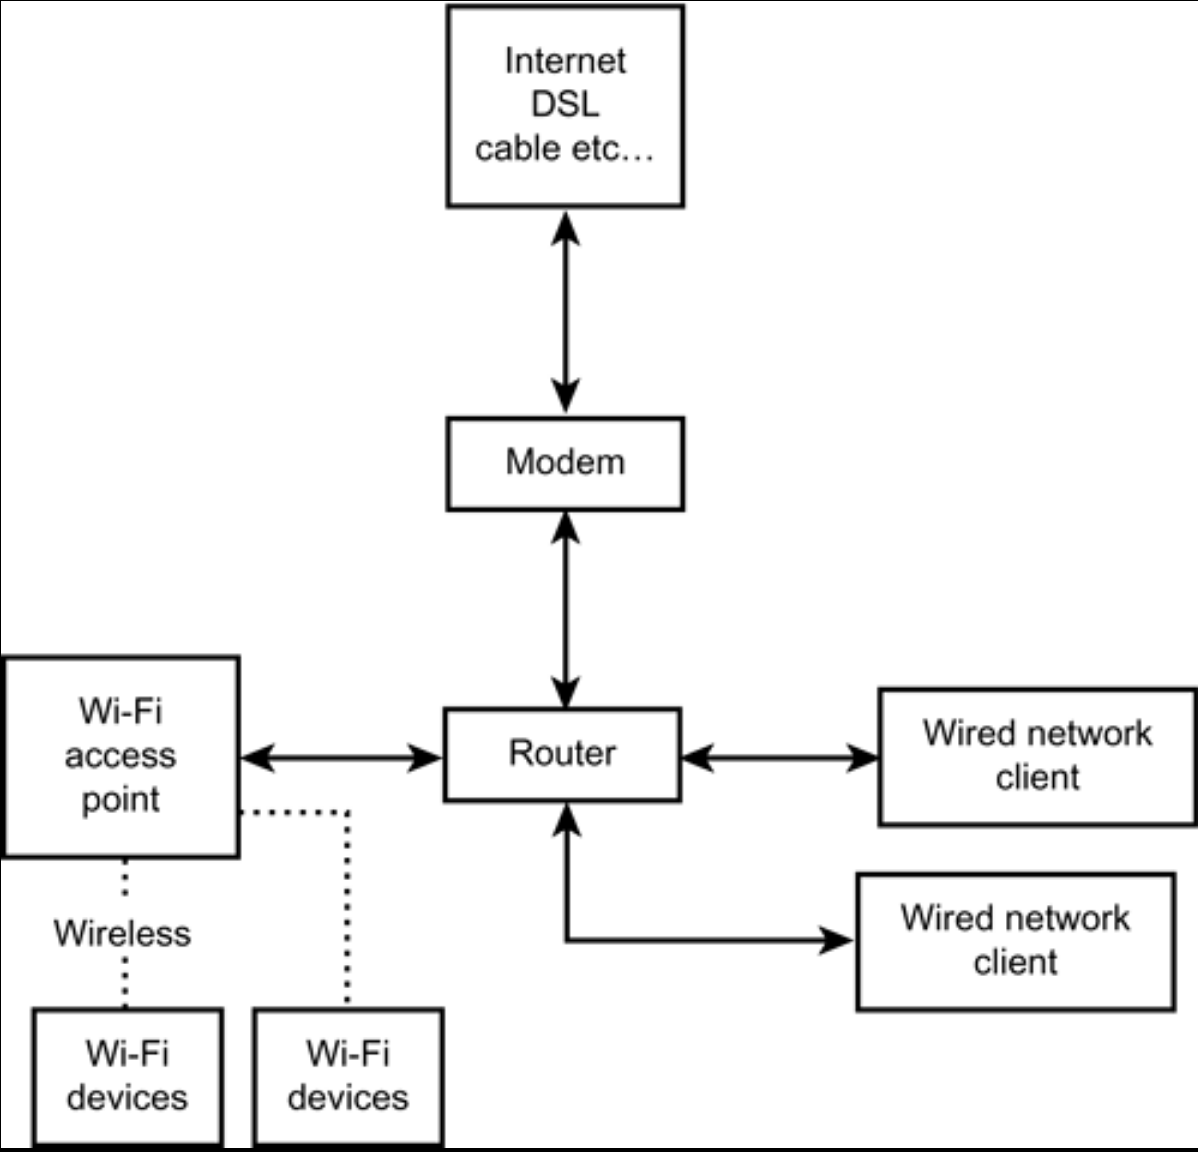
\includegraphics[width=8cm]{wifi-red-basica}
    \caption{Tomado de \cite{davis}.}
    \label{fig:wifi-red-basica}
\end{figure}


\subsection{Espectros inalámbricos}
A diferencia de mucho otros estándares inalámbricos , 802.11 funciona en porciones ``libres'' del espectro de radio. Esto significa que (a diferencia de las comunicaciones telefónicas celulares) ninguna licencia se require para transmitir o comunicarse usando 802.11 (o Wi-Fi).

Las porciones libres del espectro de rado usadas por 802.11 (y Wi-Fi) son la bandas de 2.4, 3.6, 5 y 60GHz. Teléfonos inalámbricos y otros electrodomésticos hacen uso de estos espectros libres. El estándar 802.11 y (Wi-Fi) incluye la capa física, en esta se utiliza una tecnología conocida como \emph{Direct Sequence Spread Spectrum} (DSSS) para prevenir colisiones y evitar interferencia entre los dispositivos que operan en el mismo espectro. La idea con eso es que una señal que viene de algún electrodoméstico no interfiera con la descarga de un \emph{e-mail} o viceversa. 

Además de la capa física, cada dispositivo Wi-Fi 802.11 tiene una capa de control de acceso. La capa de control de acceso especifica cómo un dispositivo Wi-Fi, como una computadora portátil, se comunica con otro dispositivo Wi-Fi, como un punto de access inalámbrico. Para proporcionar seguridad, se le ha añadido al estándar el \emph{Wi-Fi Protected Access solution} (WPA). 

En conjunto, la capa física y la capa de control de acceso, junto con extensiones dirigidas para implementar funcionalidades extra (como WPA para seguridad) han el estándar 802.11 Wi-Fi.

\subsubsection{¿Por qué Wi-Fi es importante?}
El estándar 802.11 es importante porque millones de personas alrededor del mundo están haciendo uso de él. Lo utilizan para conectarse sin cables a Internet cuando están de viaje o lejos de su casa u oficina. También se usa 8802.11 para crear redes inalámbricas en su casas y oficinas.

Wi-Fi provee garantía de compatibilidad para los dispositivos 802.11. Cada dispositivo 802.11 puede ``hablar'' con cualquier otro dispositivo Wi-Fi -- y la \emph{Wi-Fi Alliance} certifica esto. La funcionalidad y la durabilidad de cada dispositivo con el logo Wi-Fi es probado y certificado en laboratorios independientes. De igual forma, la \emph{Wi-Fi Alliance} y las compañías que la conforman están comprometidas en un esfuerzo continuo para expandir los estándares inalámbricos, y hacer de la computación inalámbrica una experiencia más segura y agradable.

\subsubsection{Los espectros libres}
Cualquier señal que se envía sin cables se le llama transmisión de radio. Cada dispositivo que transmite una transmisión por radio lo hace a una frecuencia particular. Al conjunto total de frecuencias de radio se le conoce como espectro de radio. A las porciones contiguas del espectro de rado se le llaman bandas, como ``la banda FM''.

Mil megahertz es igual a un gigahertz (GHz). Así que cuando se hace referencia a 2.4Ghz, se habla en realidad de 2 400 000 000 oscilaciones por segundo. 

Solo hay algunas frecuencias en el espectro de radio que pueden ser utilizadas para trasmisiones. Esto inevitablemente lleva a potenciales conflictos acerca de su uso así como intento por dominar frecuencias particulares. Como respuesta parcial, los gobiernos han regulado el uso de la mayoría de estas frecuencias. Algunas frecuencias están reservadas para usos particulares como en defensa militar. Otras como las bandas AM y FM se ofrecen bajo licencia. Algunas áreas del espectro se han dejado de lado para usos que no requieren licencia. Estas áreas retiradas incluyen los espectros como los de 2.4Ghz y 5Ghz que son los que usa Wi-Fi. Los usos de algunas de las frecuencias del espectro de radio se muestran en la figura \ref{fig:espectro-radio}

\begin{figure}[h]
    \centering
    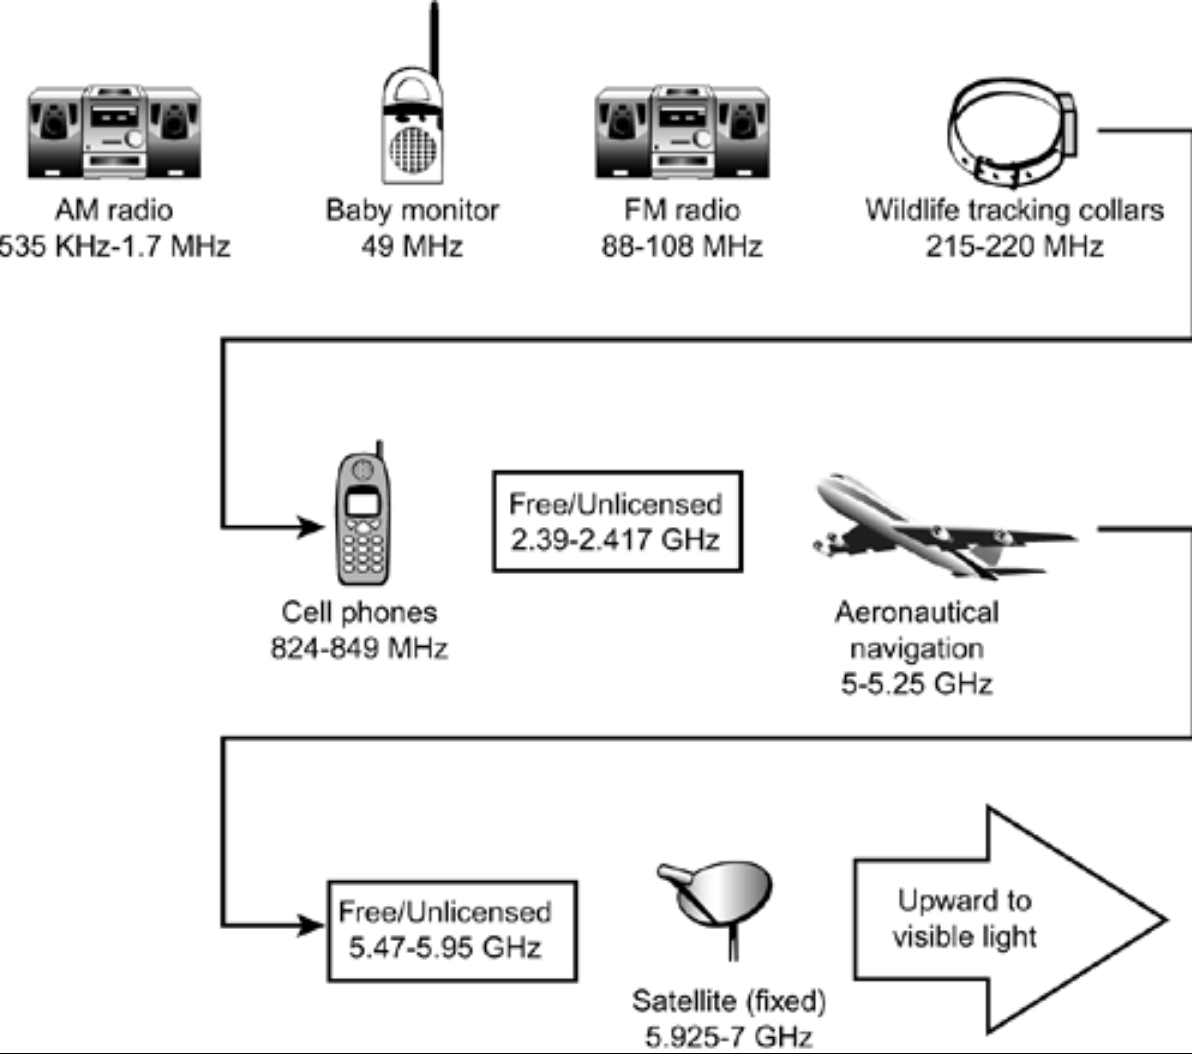
\includegraphics[width=8cm]{espectro-radio}
    \caption{Tomado de \cite{davis}.}
    \label{fig:espectro-radio}
\end{figure}

El hecho que frecuencias como 2.4Ghz y 5Ghz se hayan retirado para usos que no requieren de licenciamiento tiene una implicación muy importante: su uso es barato. Esto les brinda a estos espectros ``libres'' un ventaja competitiva injusta comparado con el uso de un espectro por el que hay que pagar. De igual forma existen restricciones legales de los que se pueda hacer y lo que no con los espectros libres.

También, al ser libre, espectros como 2.4Ghz se ha llenado de toda clase de dispositivos de transmisión, desde hornos de microondas hasta teléfonos inalámbricos. Estos dispositvos puede interferir con la transmisión Wi-Fi y su recepción.

\subsection{El estándar 802.11 y sus variantes}
En general, el núclo del estándar 802.11 está dirigido a especificar una forma en que las computadoras puedan conectarse en red (formando redes de área local) usando los espectros libres de 2.4Ghz y 5Ghz. 

Hoy en día cuando se menciona ``Wi-Fi'', probablemente signifique 802.11b, el cual es un subconjunto del estándar general 802.11. La mayoría de los dispositivos Wi-Fi que están en operación están usando 802.11b. Sin embargo, la tecnología se mueve rápidamente y otras variantes como 802.11g se están haciendo más populares.

Algunas cosas importantes a saber de 802.11b:
\begin{itemize}
    \item El estándar 802.11b usa el espectro de 2.4Ghz.
    \item El estándar 802.11b usa la tecnología de DSSS para minizar la interferencia con otros dispositivos que trasmiten en el espectro de 2.4Ghz.
    \item El estándar 802.11 brinda una velocidad teórica de 11Mbps.
\end{itemize}

En comparación, la velocidad de 11Mbps se muestra como favorable con respecto a los 10Mbps de velocidad un una red Ethernet cableada convencional \textsc{10BASE-T}. Sin embargo, por una variedad de razones, las conexiones Wi-Fi raramente alcanzan su máximo teórico. Aún así, las conexiones Wi-Fi deberían ser suficientes para el uso diario cuando se comparten archivos o se navega por Internet. 

\subsubsection{802.11a y 802.11g}
802.11a y 802.11g son variantes del estándar 802.11 que pueden ser considerados como más ``inteligentes'' que 802.11b. El estándar 802.11a usa la banda de 5Ghz para transmissión lo cual minimiza la posibilidad de interferencia con todos los dispositivos que transmiten en 2.4GHz y promete una rendimiento de 24Mbps. 

802.11g opera en la banda de 2.4GHz y cuanta con rendimiento tan rápido como 54Mbps.

En otras palabras ambos, 802.11a y 802.11g ofrecen la promesa de ser considerablemente más rápidos que 802.11b. De hecho, 802.11g está empezando a reemplazar a 802.11b como el estándar para los nuevos equipos. Existen otros estándares como 802.11n, el cual se postula con un nuevo competidor para los anteriores. En \cite{wikipedia-80211} se mantiene una lista detallada de las variantes de 802.11 conocidas hasta la fecha. 


\subsubsection{Velocidades de transmisión}
En la figura \ref{fig:wifi-velocidades} se muestra una comparación de las velocidades de los estándares inalámbricos. 802.11b Wi-Fi es un poco más lento que una red cableada pero es más adecuada para pequeñas oficinas y casas.

\begin{figure}[h]
    \centering
    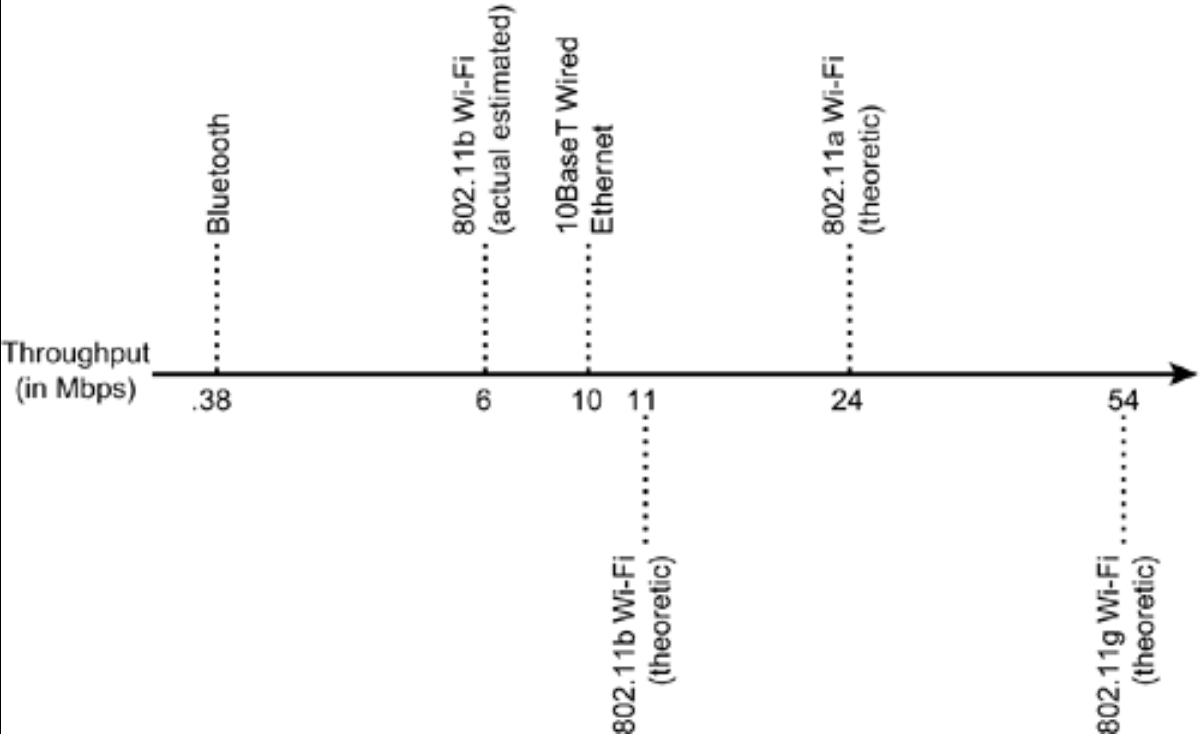
\includegraphics[width=9cm]{wifi-velocidades}
    \caption{Tomado de \cite{davis}.}
    \label{fig:wifi-velocidades}
\end{figure}

\section{WiMAX}
WiMAX es la abreviación para \emph{Worldwide Interoperability for Microwave Accesss} y fue introducido en el 2001. Su propósito era promover la conformidad e interoperatibilidad del estándar oficial IEEE 802.11 llamado \emph{``Wireless MAN''}. WiMAX está basado en el estándar IEEE 802.16 (tal y como se muestra en la figura \ref{fig:wimax-standards}) . Esta tecnología está principalmente asociada como una tecnología de conectividad de ``última milla'' (\emph{last mile})  de alta velocidad. Las tecnologías de banda ancha como Wi-Fi usan ADSL como su red apoyo (\emph{backbone}), sin embargo, WiMAX usa tecnología inalámbrica, haciéndola accesible incluso en áreas en donde no están conectadas por cable o fibra.

\begin{figure}[h]
    \centering
    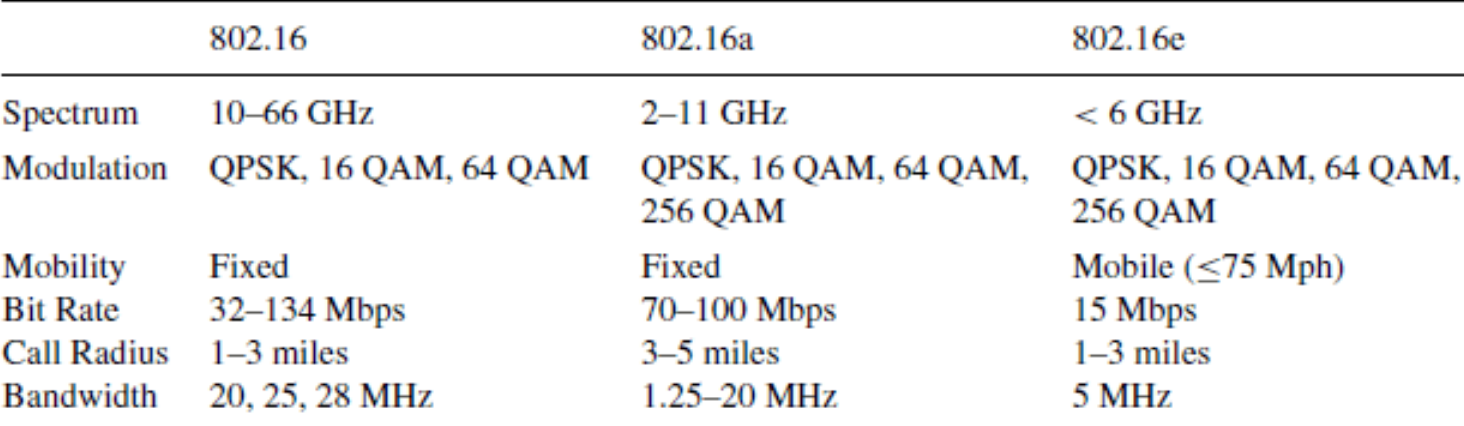
\includegraphics[width=9cm]{wimax-standards}
    \caption{Algunos estándares 802.11 para WiMAX \cite{mishra}.}
    \label{fig:wimax-standards}
\end{figure}

\begin{table}[h!]
    \centering
    \begin{tabular}{l|l|l}
        \toprule[1.5pt]
         & \textbf{\emph{Fixed} WiMAX} & \textbf{\emph{Mobile} WiMAX}\\
        \midrule
        Tipo de Red & \emph{Fixed} & \emph{Fixed, Mobile} \\
        Modulación & OFDM & OFDMA \\
        Frecuencia & 2.5, 3.4-3.6, 5.8GHz & 2.3-2.4, 2.5-2.7,\\
                   &                      &3.3-3.4, 3.4-3.8GHz\\
        Duplex & TDD, FDD & TDD, FDD \\
        \emph{Handoff} & No & Sí \\
        Equipo & \emph{Outdoor/Indoor} CPE & CPE, módulos integrados \\
        \bottomrule[1.5pt]
    \end{tabular}
    \caption{\emph{Fixed} vs \emph{Mobile} WiMAX}
    \label{table:fixed-mobile}
\end{table}

Las principales ventajas de WiMAX sobre sobre sistemas son:
\begin{itemize}
    \item Mejor rendimiento del sistema gracias a mecanismos avanzados de QoS.
    \item Mayor rendimiento debido a las robustas tecnologías de adaptación y eficiencia espectral (casi tres veces mejor que los actuales sistemas 3G).
    \item Capacidad para rellenar los vacíos (debido a la conexión inalámbrica) en una región que tiene banda ancha debido a cable/DSL.
    \item Interoperatibilidad
    \item Tiene la habilidad de ``banda ancha bajo demanda'', con anchos de banda de hasta 100Mbps.
    \item El diseño del sistem no necesita condiciones de ``línea de vista'' 
\end{itemize}


El rendimiento de los sistemas WiMAX se debe al uso de las tecnologías de interface aérea OFDM y OFDMA. La utilización de TDD (\emph{Time Division Duplex}) también mejora el rendimiento del sistema, aunque FDD (\emph{Frequency Division Duplex}) también se puede usar. Gracias a estas técnicas de multiplexación, altas tasas de datos puede ser ofrecidos a los subscriptores con una mayor eficiencia espectral. Debido a 802.16, la calidad del servicio es mayor en el sistema. Las características de MAC permiten una QoS basada en IP \emph{e2e}, ya que proporciona flexibilidad en la programación de los recursos a través de la interfaz aérea. La red WiMAX es más interoperable que el resto de las redes BWA (\emph{Broadband Wireless Access}). Las frecuencias se encuentran en en rangos que van desde 2.3GHz, 2.5GHz y 3.4-3.8GHz para bandas con licencia y 5.8GHz en bandas sin licencia. Aunque las bandas sin licencia parecen ser la mejor opción, existen problemas asociadas con las mismas, por ejemplo, interferencia: una gran cantidad de interferencia puede esperarse de otras tecnologías que puedan usar esta banda, por ejemplo \emph{Bluetooth} o Wi-Fi. Latencia, seguridad y regulaciones del espectro son también algunos de los problemas que se pueden presentar.

Las características principales de los sistemas WiMAX son:
\begin{itemize}
    \item WiMAX es un sistema TDD.
    \item Los requerimientos del espectro van desde 10MHz a 30MHz
    \begin{itemize}
        \item Banda de frecuencia: Licenciada 2.5/2.5 GHz; 3.5GHz
        \item Banda de frecuencia: Sin licencia 5.8 GHz
    \end{itemize}
    \item Estimaciones de rendimiento:
    \begin{itemize}
        \item Teórico: 70Mbps (para una portadora de 20MHz)
    \end{itemize}
    \item Rango celular
    \begin{itemize}
        \item Para 2.5GHz, 500m - 1.5Km
    \end{itemize}
\end{itemize}

\subsection{OFMDA: Modulación en WiMAX}
\emph{Mobile} WiMAX adopta \emph{Orthogonal Frequency Division Multiple Access} (OFDMA) para un rendimiento \emph{multi-path} mejorado en ambientes ``fuera de la línea de vista''. OFDMA escalable fue introducido como una enmienda para soportar anchos de banda de canales escalables de 1.25 a 20 MHz. El grupo técnico móvil del WiMAX forum está desarrollando perfiles de sistemas WiMAX móviles que van a definirá las características obligatorias y opcionales de la norma IEEE. El perfil habilita que los sistemas móviles sean configurados basados en un conjunto de base de funcionalidad. 

Esta es una técnica de multiplexación que subdivide el ancho de banda en múltiples frecuencias sub-portadoras. En este sistema, los flujos de datos de entrada se divide en varias sub-flujos paralelos de tasas de datos reducidos que son modulado y transmitidos en una sub-portadora ortogonal como se muestra en la figura \ref{fig:ofdma}.

\begin{figure}[h]
    \centering
    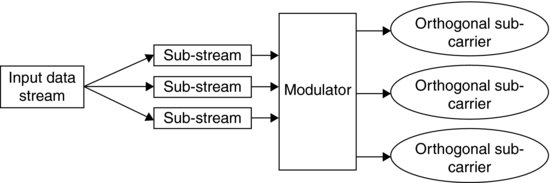
\includegraphics[width=9cm]{ofdma}
    \caption{Arquitectura de OFDMA \cite{mishra}.}
    \label{fig:ofdma}
\end{figure}

\subsection{Arquitectura de WiMAX}
Un diagrama de bloques simplificado de la red WiMAX se muestra en la figura \ref{fig:wimax-architecture}. La red WiMAX consiste de 3 principales aspectos:
\begin{itemize}
    \item Estación móvil / Equipo
    \item Red de servicios de acceso (\emph{Access Services Network} - ASN)
    \item Red de servicios de conectividad (\emph{Connectivity Services Network} - CSN)
\end{itemize}


\begin{figure}[h]
    \centering
    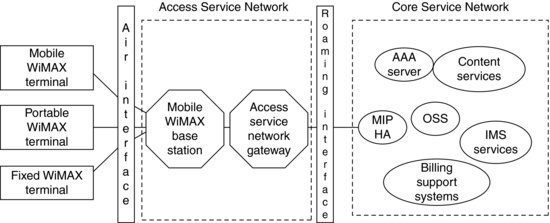
\includegraphics[width=9cm]{wimax-architecture}
    \caption{Arquitectura de OFDMA \cite{mishra}.}
    \label{fig:wimax-architecture}
\end{figure}

\subsubsection{Estación Móvil}
La estación móvil como en otras red conecta al usuario a la estación base o al acceso a la red. La principal diferencia con dispositivos GSM o CDMA es que estos necesitan ser compatibles con IEEE 802.16. También, el dispositivo móvil debe tener funcionalidades como gestión de recursos, gestión móvil, capacidad de ahorro de energía, autorización, autenticación y gestión de sesiones.

\subsubsection{Red de servicios de acceso}
La red de servicios de acceso conecta el subscriptor móvil al IP \emph{backbone} usando la interface aérea OFDMA. Consiste principalmente de dos partes: la estación base y el ASN \emph{Gateway}. Un ASN puede consistir de uno o mas estaciones base y uno o más ASN \emph{gateways}.

\paragraph{Estación base} un diagrama simplificado de la estación base se muestra en la figura \ref{fig:base-station}. Tiene un módulo de radio frecuencia y un módulo de sistema. En práctica, hay más de un módulo de radio frecuencia en las estaciones base. Ambos módulos están conectados a un cable óptico \emph{Open Base Station Architecture Initiative}

\begin{figure}[h]
    \centering
    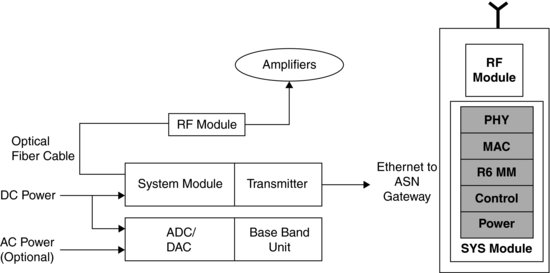
\includegraphics[width=9cm]{base-station}
    \caption{Estación base WiMAX \cite{mishra}.}
    \label{fig:base-station}
\end{figure}

Como el nombre lo indica, las funciones de radio frecuencia son realizads por el módulo de radio frecuencia. El módulo de radio frecuencia tiene interfaces hacia el módulo del sistema, energía y sistema de antena. El módulo del sistema es responsable por el control de la estación base y realiza funciones relacionadas a la capa física (transmisión y recepción de símbolos ODFM, control de energía, etc) y la capa MAC (configuración de conectividad, \emph{scheduling}, movilidad, etc).

\paragraph{ASN Gateway} como se muestra en la figura \ref{fig:wimax-architecture} es una interface entre ASN y CSN. El ASN \emph{gateway} es una entidad lógica que es responsable de funciones como gestión móvil, por ejemplo, paginación (\emph{paging}), QoS, interfaz de interceptación legal, autenticador, gestión de flujos de datos, etc. La ASN \emph{gateway} realiza principalmente una o muchas de las tareas de plano de control, plano de usuario y \emph{gateway} de servicio y destino.

\paragraph{Red de servicios de conectividad (CSN)} realiza algunas funciones clave en una red WiMAX. Como el nombre lo sugiere, provee conectividad para las redes externas como Internet, PLMN y otras. También proporciona políticas de contro para voz y VPN. Es también responsable de gestión de direcciones IP (DHCP, AAA, etc) y localización, además de gestión de movilidad entre los ASNs. El CSN es también responsable de la gestión de QoS. El CSN contiene dos elementos principales:
\begin{itemize}
    \item Servidor de autenticación, autorización y bitácora (\emph{Authentication, Authorization and Accounting} - AAA).
    \item Agente Doméstico (\emph{Home Agent} - HA)
\end{itemize}


% needed in second column of first page if using \IEEEpubid
%\IEEEpubidadjcol


% An example of a floating figure using the graphicx package.
% Note that \label must occur AFTER (or within) \caption.
% For figures, \caption should occur after the \includegraphics.
% Note that IEEEtran v1.7 and later has special internal code that
% is designed to preserve the operation of \label within \caption
% even when the captionsoff option is in effect. However, because
% of issues like this, it may be the safest practice to put all your
% \label just after \caption rather than within \caption{}.
%
% Reminder: the "draftcls" or "draftclsnofoot", not "draft", class
% option should be used if it is desired that the figures are to be
% displayed while in draft mode.
%
%\begin{figure}[!t]
%\centering
%\includegraphics[width=2.5in]{myfigure}
% where an .eps filename suffix will be assumed under latex, 
% and a .pdf suffix will be assumed for pdflatex; or what has been declared
% via \DeclareGraphicsExtensions.
%\caption{Simulation results for the network.}
%\label{fig_sim}
%\end{figure}

% Note that IEEE typically puts floats only at the top, even when this
% results in a large percentage of a column being occupied by floats.
% However, the Computer Society has been known to put floats at the bottom.


% An example of a double column floating figure using two subfigures.
% (The subfig.sty package must be loaded for this to work.)
% The subfigure \label commands are set within each subfloat command,
% and the \label for the overall figure must come after \caption.
% \hfil is used as a separator to get equal spacing.
% Watch out that the combined width of all the subfigures on a 
% line do not exceed the text width or a line break will occur.
%
%\begin{figure*}[!t]
%\centering
%\subfloat[Case I]{\includegraphics[width=2.5in]{box}%
%\label{fig_first_case}}
%\hfil
%\subfloat[Case II]{\includegraphics[width=2.5in]{box}%
%\label{fig_second_case}}
%\caption{Simulation results for the network.}
%\label{fig_sim}
%\end{figure*}
%
% Note that often IEEE papers with subfigures do not employ subfigure
% captions (using the optional argument to \subfloat[]), but instead will
% reference/describe all of them (a), (b), etc., within the main caption.
% Be aware that for subfig.sty to generate the (a), (b), etc., subfigure
% labels, the optional argument to \subfloat must be present. If a
% subcaption is not desired, just leave its contents blank,
% e.g., \subfloat[].


% An example of a floating table. Note that, for IEEE style tables, the
% \caption command should come BEFORE the table and, given that table
% captions serve much like titles, are usually capitalized except for words
% such as a, an, and, as, at, but, by, for, in, nor, of, on, or, the, to
% and up, which are usually not capitalized unless they are the first or
% last word of the caption. Table text will default to \footnotesize as
% IEEE normally uses this smaller font for tables.
% The \label must come after \caption as always.
%
%\begin{table}[!t]
%% increase table row spacing, adjust to taste
%\renewcommand{\arraystretch}{1.3}
% if using array.sty, it might be a good idea to tweak the value of
% \extrarowheight as needed to properly center the text within the cells
%\caption{An Example of a Table}
%\label{table_example}
%\centering
%% Some packages, such as MDW tools, offer better commands for making tables
%% than the plain LaTeX2e tabular which is used here.
%\begin{tabular}{|c||c|}
%\hline
%One & Two\\
%\hline
%Three & Four\\
%\hline
%\end{tabular}
%\end{table}


% Note that the IEEE does not put floats in the very first column
% - or typically anywhere on the first page for that matter. Also,
% in-text middle ("here") positioning is typically not used, but it
% is allowed and encouraged for Computer Society conferences (but
% not Computer Society journals). Most IEEE journals/conferences use
% top floats exclusively. 
% Note that, LaTeX2e, unlike IEEE journals/conferences, places
% footnotes above bottom floats. This can be corrected via the
% \fnbelowfloat command of the stfloats package.




\section{Conclusión}





% if have a single appendix:
%\appendix[Proof of the Zonklar Equations]
% or
%\appendix  % for no appendix heading
% do not use \section anymore after \appendix, only \section*
% is possibly needed

% use appendices with more than one appendix
% then use \section to start each appendix
% you must declare a \section before using any
% \subsection or using \label (\appendices by itself
% starts a section numbered zero.)
%


%\appendices
%\section{Proof of the First Zonklar Equation}
%Appendix one text goes here.
%
%\section{}
%Appendix two text goes here.


% use section* for acknowledgment
%\ifCLASSOPTIONcompsoc
%  % The Computer Society usually uses the plural form
%  \section*{Acknowledgments}
%\else
%  % regular IEEE prefers the singular form
%  \section*{Acknowledgment}
%\fi


%The authors would like to thank...


% Can use something like this to put references on a page
% by themselves when using endfloat and the captionsoff option.
\ifCLASSOPTIONcaptionsoff
  \newpage
\fi



% trigger a \newpage just before the given reference
% number - used to balance the columns on the last page
% adjust value as needed - may need to be readjusted if
% the document is modified later
%\IEEEtriggeratref{8}
% The "triggered" command can be changed if desired:
%\IEEEtriggercmd{\enlargethispage{-5in}}

% references section

% can use a bibliography generated by BibTeX as a .bbl file
% BibTeX documentation can be easily obtained at:
% http://www.ctan.org/tex-archive/biblio/bibtex/contrib/doc/
% The IEEEtran BibTeX style support page is at:
% http://www.michaelshell.org/tex/ieeetran/bibtex/
%\bibliographystyle{IEEEtran}
% argument is your BibTeX string definitions and bibliography database(s)
%\bibliography{IEEEabrv,../bib/paper}
%
% <OR> manually copy in the resultant .bbl file
% set second argument of \begin to the number of references
% (used to reserve space for the reference number labels box)
\begin{thebibliography}{1}

\bibitem{davis}
H.~Davis. \emph{Absolute Beginner's Guide to Wi-Fi Wireless Networking}. \hskip 1em plus 0.5em minus 0.4em\relax Que. ISBN: 0789731150. Abril, 2004.

\bibitem{mishra}
A.R.~Mishra. \emph{Cellular Technologies for Emerging Markets: 2G, 3G and Beyond}. \hskip 1em plus 0.5em minus 0.4em\relax John Wiley and Sons. ISBN: 9780470779477. Agosto 2010.

\bibitem{wikipedia-80211}
Wikipedia. IEEE 802.11. Disponible en \url{https://en.wikipedia.org/wiki/IEEE_802.11}

  
\end{thebibliography}

% biography section
% 
% If you have an EPS/PDF photo (graphicx package needed) extra braces are
% needed around the contents of the optional argument to biography to prevent
% the LaTeX parser from getting confused when it sees the complicated
% \includegraphics command within an optional argument. (You could create
% your own custom macro containing the \includegraphics command to make things
% simpler here.)
%\begin{IEEEbiography}[{\includegraphics[width=1in,height=1.25in,clip,keepaspectratio]{mshell}}]{Michael Shell}
% or if you just want to reserve a space for a photo:

\begin{IEEEbiography}[{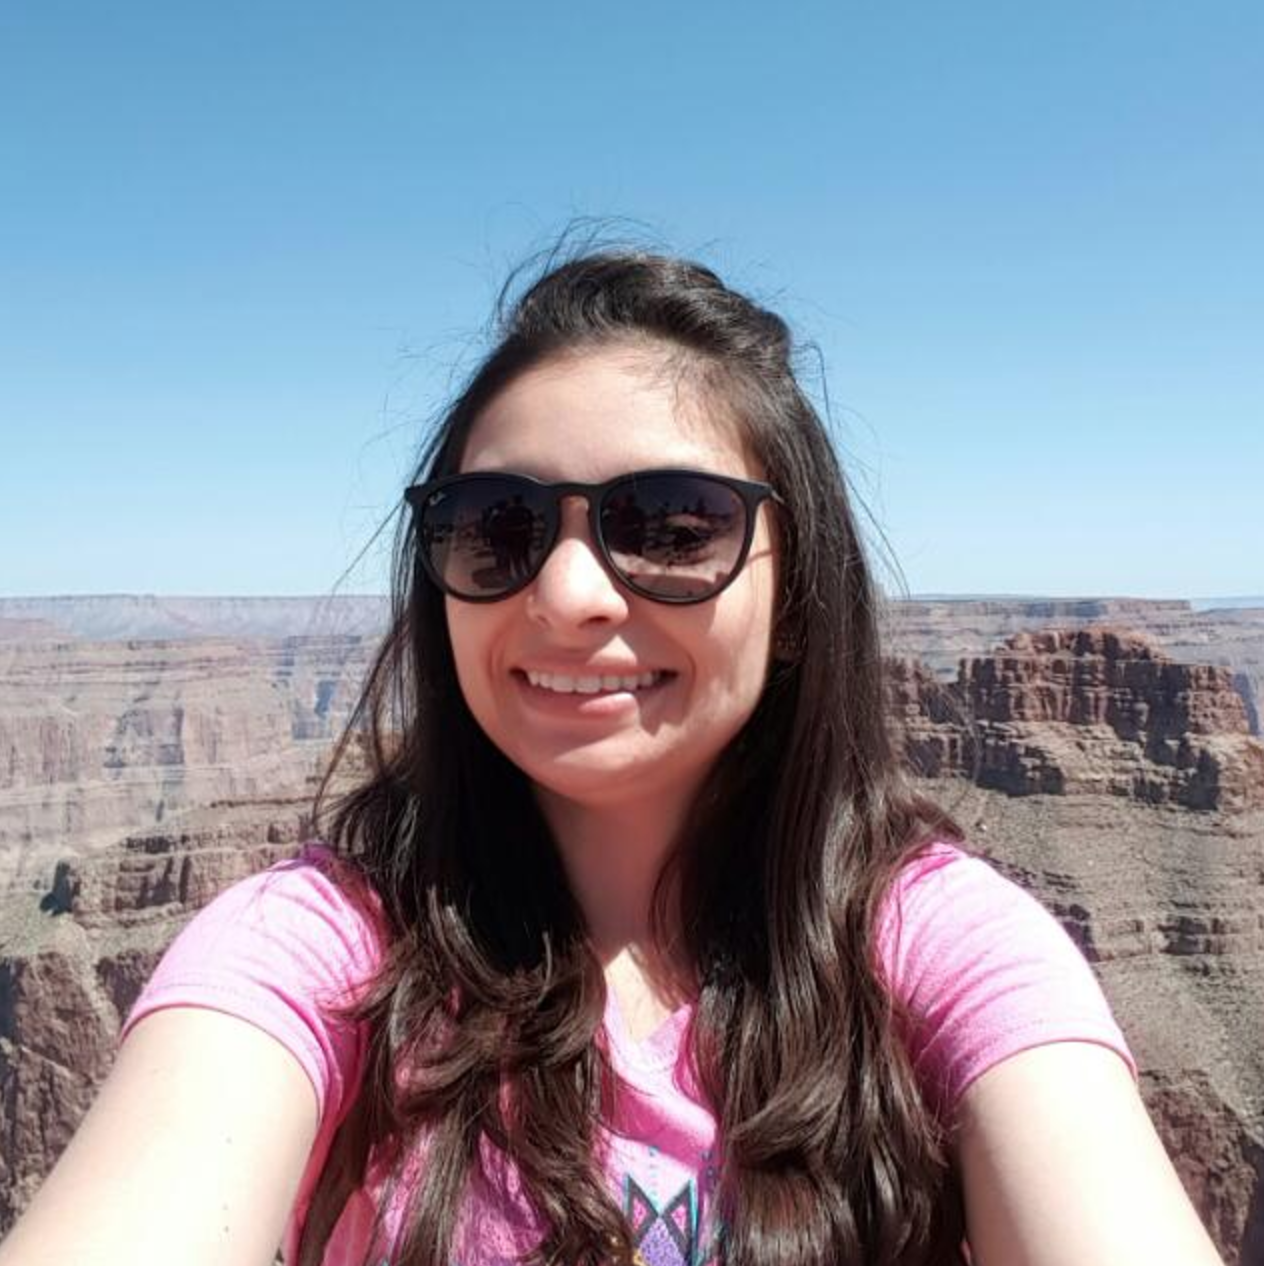
\includegraphics[width=1in,height=1.25in,clip,keepaspectratio]{priscilla-piedra}}]{Priscilla Piedra}
es Ingeniera de Computación del Tecnologíco de Costa Rica. Actualmente es estudiante del programa de Maestría en Ciencas de la Computación en la misma universidad. Sus principales intereses son: \emph{cloud computing} y automatización. 
\end{IEEEbiography}

% if you will not have a photo at all:
\begin{IEEEbiography}[{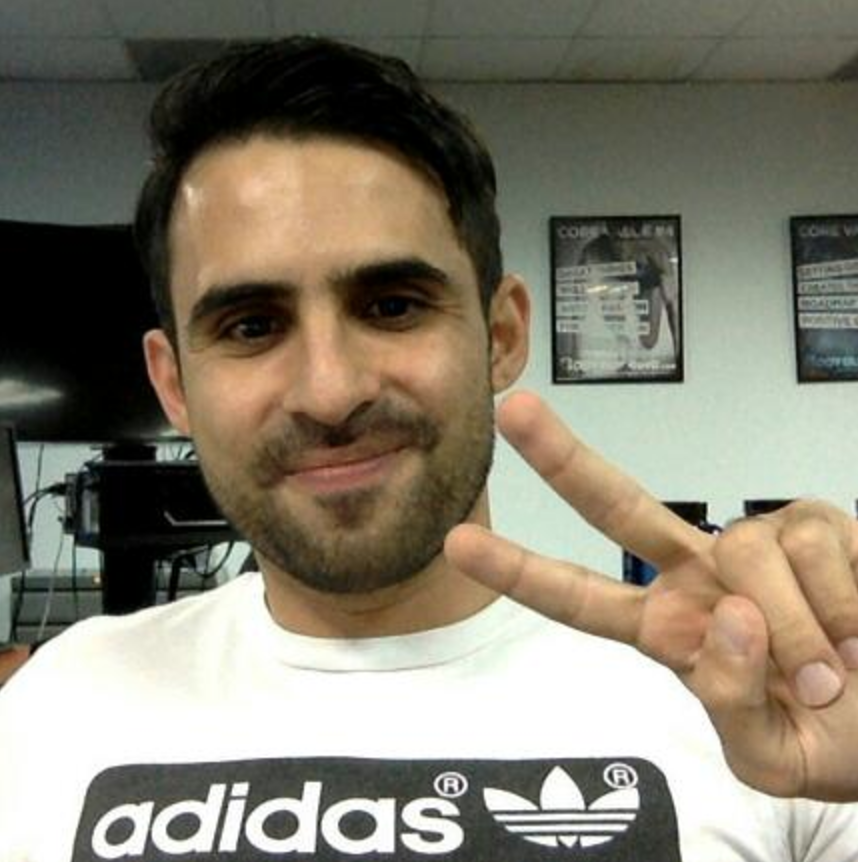
\includegraphics[width=1in,height=1.25in,clip,keepaspectratio]{martin-flores}}]{Martín Flores}
es Ingeniero en Informática de la Universidad Nacional. Actualmente, realiza sus estudios de Maestría en Ciencias de la Computación del Tecnológico de Costa Rica. Sus principales intereses son: lenguajes de programación, ingeniería de software y \emph{DevOps}.
\end{IEEEbiography}

% insert where needed to balance the two columns on the last page with
% biographies
%\newpage

%\begin{IEEEbiographynophoto}{Jane Doe}
%Biography text here.
%\end{IEEEbiographynophoto}

% You can push biographies down or up by placing
% a \vfill before or after them. The appropriate
% use of \vfill depends on what kind of text is
% on the last page and whether or not the columns
% are being equalized.

\vfill

% Can be used to pull up biographies so that the bottom of the last one
% is flush with the other column.
%\enlargethispage{-5in}



% that's all folks
\end{document}


